\section{Results}
\label{sec:results}

%% Revised 2026-08-30 against the GPT-5.6-Sol review and tightened for the page budget. Every
%% detection headline names an autonomous row; curated C# scores are upper bounds; "lead" is the
%% defined strict rule; post-hoc pairs reported; A5 read at the operating point; RQ6 gains the
%% combined and real-history arms; RQ9's R1-vs-R2 row is inter-rater agreement. Macros only.
%% 2026-09-13 shortening pass (response plan §13): every result stays; the diagnostic's
%% sensitivity intervals (M4), the full inferential detail (M5), the SARIF/FCA numbers (M10),
%% the per-operator, combined-loss and per-pair history drift tables (M1, M2), the
%% rater-agreement forensics and the effort table (M3, M8) moved to the TR, each replaced by its
%% compact form. The caveats the terms box / §IV / §VII carry are not restated here.
%% 2026-09-13 readability pass: the RQ2 and RQ7 paragraphs split into three each, long sentences
%% split; every macro, number, and citation unchanged.

\subsection{RQ1: Recoverability, diagnosed without the reference}
\label{sec:rq1}
%% GENERATED by analysis/make_tables.py from results.csv -- DO NOT EDIT BY HAND.
\begin{table*}[t]
  \centering
  \caption{Corpus, RQ1 fidelity, and the A1/A5 ablation columns (terms: \S\ref{sec:design}). \#Cl./\#Ent./\#Tgt.\ = reference clusters, scored entities, first-party targets; Best = best all-common classical baseline by MoJoFM; A1 = container edges at L0 $\to$ all layers; A5 = container edges the never-drop-declared rule saves at threshold 3 / 8. GT-diag = inception-era diagram, architect-reconciled (P-1 curated with that diagram in view); $^\ddagger$anonymized proprietary system, non-replicable, corroborating only (entity count bucketed). P-1 floor/propose: its A2 rungs. $^\S$Squidex's only curated model is its reference-blind RQ7 curation.}
  \label{tab:corpus}\label{tab:rq1}\label{tab:rq3}
  \footnotesize\setlength{\tabcolsep}{3pt}
  \begin{tabular}{@{}lllll rrr rr rr rr r rr@{}}
    \toprule
    & & & & & & & & \multicolumn{2}{c}{Floor} & \multicolumn{2}{c}{Propose} & \multicolumn{2}{c}{Curated} & Best & A1 & A5 \\
    \cmidrule(lr){9-10}\cmidrule(lr){11-12}\cmidrule(lr){13-14}
    System & Lang & Build & Ref & Cur. & \#Cl. & \#Ent. & \#Tgt. & a2a & MoJo & a2a & MoJo & a2a & MoJo & MoJo & edges & t3/t8 \\
    \midrule
    ITK & C++ & CMake & GT-pub & assisted & 13 & 7657 & 79 & 84.2 & 96.9 & 97.8 & 98.3 & 99.6 & 98.4 & 93.9 & 17$\to$23 & 0/5 \\
    abseil & C++ & CMake & GT-exp & assisted & 21 & 809 & 190 & 85.1 & 89.9 & 100.0 & 100.0 & 98.8 & 95.2 & 97.8 & 79$\to$83 & 0/45 \\
    OpenCV & C++ & CMake & GT-doc & assisted & 14 & 1087 & 24 & 100.0 & 100.0 & 87.0 & 48.3 & 100.0 & 100.0 & 92.1 & 9$\to$9 & 0/5 \\
    bash & C & Makefile.in & GT-pub & assisted & 14 & 373 & 49 & 97.7 & 91.9 & 95.3 & 82.7 & 98.1 & 93.2 & 91.9 & 8$\to$17 & 0/5 \\
    libxml2 & C & automake & GT-pub & none & 18 & 82 & 14 & 76.0 & 11.4 & 73.5 & 5.7 & 76.0 & 11.4 & 31.4 & 3$\to$3 & 0/3 \\
    eShop & C\# & .NET SDK & GT-doc & sighted & 9 & 19 & 19 & 80.8 & 33.3 & 73.3 & 0.0 & 88.9 & 66.7 & 33.3 & 30$\to$30 & 0/30 \\
    OrchardCore & C\# & .NET SDK & GT-doc & sighted & 34 & 207 & 207 & 67.6 & 11.6 & 91.1 & 69.5 & 91.7 & 72.1 & 47.4 & 70$\to$72 & 0/26 \\
    nopCommerce & C\# & .NET SDK & GT-doc & sighted & 17 & 37 & 37 & 80.2 & 37.5 & 89.6 & 71.9 & 90.2 & 71.9 & 46.9 & 16$\to$30 & 0/0 \\
    Squidex$^\S$ & C\# & .NET SDK & GT-exp & blind & 12 & 15 & 26 & 92.0 & 70.0 & 86.8 & 50.0 & 95.8 & 70.0 & 70.0 & -- & -- \\
    P-1$^\ddagger$ & C++ & -- & GT-diag & sighted & 28 & 50-100 & 52 & 93.7 & 96.9 & 81.2 & 24.5 & 100.0 & 100.0 & 91.3 & -- & -- \\
    \bottomrule
  \end{tabular}
\end{table*}

%% Tables II/III anchored here (2026-09-13): same float-deferral reason as Fig. 1.
%% GENERATED by analysis/make_tables.py from results.csv -- DO NOT EDIT BY HAND.
\begin{table*}[t]
  \centering
  \caption{RQ2: MoJoFM (top) and a2a (bottom) vs.\ the reference on the all-common projection, best per row in bold. Strict wins against the five all-common baselines: curated 6 of 9 systems on MoJoFM and 7 of 9 on a2a; floor 2 of 9 and 2 of 9; propose 4 of 9 and 4 of 9. $^\dagger$ARC on its own covered subset. $^\S$LLM, mean $\pm$ sd of five reruns; -- = refused or not run. $^\ddagger$Anonymized proprietary system, non-replicable, corroborating only. P-1 floor/propose: its A2 rungs.}
  \label{tab:rq2}
  \footnotesize\setlength{\tabcolsep}{4pt}
  \begin{tabular}{@{}lrrrrrrrrrr@{}}
    \toprule
    System & Floor & Prop. & Curated & ACDC & ARC$^\dagger$ & WCA & LIMBO & dir & cc & LLM$^\S$ \\
    \midrule
    ITK & 96.9 & 98.3 & \textbf{98.4} & 70.3 & 49.2 & -- & -- & 93.9 & 48.4 & -- \\
    abseil & 89.9 & \textbf{100.0} & 95.2 & 41.1 & 25.1 & 31.2 & 35.1 & 97.8 & 19.5 & 98.8$\pm$0.2 \\
    OpenCV & \textbf{100.0} & 48.3 & \textbf{100.0} & 81.7 & 28.7 & 25.9 & 46.9 & 92.1 & 25.4 & \textbf{100.0}$\pm$0.0 \\
    bash & 91.9 & 82.7 & \textbf{93.2} & 60.5 & 32.3 & 52.8 & 51.6 & 91.9 & 62.5 & 84.2$\pm$1.6 \\
    libxml2 & 11.4 & 5.7 & 11.4 & 20.0 & 36.9 & 31.4 & 28.6 & 5.7 & 25.7 & \textbf{62.8}$\pm$1.1 \\
    eShop & 33.3 & 0.0 & 66.7 & 6.7 & 33.3 & 20.0 & 26.7 & 33.3 & 6.7 & \textbf{86.7}$\pm$4.2 \\
    OrchardCore & 11.6 & 69.5 & \textbf{72.1} & 24.2 & 40.8 & 32.6 & 47.4 & 11.6 & 24.2 & 30.2$\pm$1.3 \\
    nopCommerce & 37.5 & \textbf{71.9} & \textbf{71.9} & 28.1 & 56.2 & 46.9 & 34.4 & 37.5 & 28.1 & 60.6$\pm$3.2 \\
    Squidex & 70.0 & 50.0 & 70.0 & 0.0 & 50.0 & 50.0 & 60.0 & 70.0 & 0.0 & \textbf{76.0}$\pm$13.6 \\
    P-1$^\ddagger$ & 96.9 & 24.5 & \textbf{100.0} & 64.7 & 16.1 & 12.9 & 22.5 & 91.3 & 12.3 & -- \\
    \midrule
    System (a2a) & Floor & Prop. & Curated & ACDC & ARC$^\dagger$ & WCA & LIMBO & dir & cc & LLM$^\S$ \\
    \midrule
    ITK & 84.2 & 97.8 & \textbf{99.6} & 73.2 & 81.3 & -- & -- & 80.4 & 85.5 & -- \\
    abseil & 85.1 & \textbf{100.0} & 98.8 & 83.0 & 81.9 & 82.8 & 81.5 & 90.0 & 79.9 & 97.6$\pm$0.1 \\
    OpenCV & \textbf{100.0} & 87.0 & \textbf{100.0} & 86.3 & 82.3 & 81.2 & 84.7 & 86.6 & 81.4 & \textbf{100.0}$\pm$0.0 \\
    bash & 97.7 & 95.3 & \textbf{98.1} & 80.7 & 84.0 & 89.0 & 85.1 & 97.0 & 90.5 & 92.6$\pm$0.2 \\
    libxml2 & 76.0 & 73.5 & 76.0 & 76.6 & 87.0 & 84.2 & 82.0 & 73.5 & 78.0 & \textbf{91.3}$\pm$0.3 \\
    eShop & 80.8 & 73.3 & 88.9 & 75.9 & 89.4 & 86.0 & 85.9 & 80.8 & 75.9 & \textbf{97.9}$\pm$0.7 \\
    OrchardCore & 67.6 & 91.1 & \textbf{91.7} & 80.2 & 85.1 & 82.0 & 83.6 & 67.6 & 79.0 & 81.8$\pm$0.5 \\
    nopCommerce & 80.2 & 89.6 & 90.2 & 76.5 & 90.1 & \textbf{90.7} & 87.8 & 80.2 & 76.5 & 84.2$\pm$12.3 \\
    Squidex & 92.0 & 86.8 & 95.8 & 69.8 & 88.4 & 88.4 & 93.0 & 92.0 & 69.8 & \textbf{96.1}$\pm$1.4 \\
    P-1$^\ddagger$ & 93.7 & 81.2 & \textbf{100.0} & 88.5 & 79.5 & 78.4 & 81.3 & 87.3 & 78.2 & -- \\
    \bottomrule
  \end{tabular}
\end{table*}

%% GENERATED by analysis/make_tables.py from results.csv -- DO NOT EDIT BY HAND.
\begin{table*}[t]
  \centering
  \caption{Cluster count $k$ (left; Ref = reference clusters; -- = not recorded) and post-hoc ARI ($\times$100, right; best per row in bold; $^\S$mean $\pm$ sd of the LLM reruns) of every partition in Tables~\ref{tab:rq1} and~\ref{tab:rq2}. $^\dagger$ARC on its own covered subset. $^\ddagger$Anonymized proprietary system, non-replicable, corroborating only. P-1 floor/propose: its A2 rungs.}
  \label{tab:rq2k}
  \scriptsize\setlength{\tabcolsep}{2.5pt}
  \begin{tabular}{@{}l r r r r r r r r r r@{}}
    \toprule
    System & Ref & Floor & Prop. & Cur. & ACDC & ARC$^\dagger$ & WCA & LIMBO & dir & cc \\
    \midrule
    ITK & 13 & 78 & 8 & 8 & 1034 & -- & -- & -- & 212 & 46 \\
    abseil & 21 & 90 & 15 & 14 & 27 & -- & 20 & 20 & 31 & 1 \\
    OpenCV & 14 & 14 & 2 & 14 & 108 & -- & 8 & 13 & 86 & 3 \\
    bash & 14 & 16 & 6 & 10 & 54 & 12 & 13 & 12 & 11 & 7 \\
    libxml2 & 18 & 3 & 1 & 3 & 4 & 13 & 10 & 9 & 1 & 2 \\
    eShop & 9 & 19 & 1 & 14 & 2 & -- & 8 & 7 & 19 & 2 \\
    OrchardCore & 34 & 201 & 20 & 16 & 13 & -- & 34 & 33 & 201 & 1 \\
    nopCommerce & 17 & 37 & 8 & 9 & 1 & -- & 17 & 16 & 37 & 1 \\
    Squidex & 12 & 13 & 6 & 10 & 1 & 7 & 7 & 9 & 13 & 1 \\
    P-1$^\ddagger$ & 28 & 49 & 6 & 27 & 52 & 13 & 2 & 18 & 86 & 1 \\
    \bottomrule
  \end{tabular}\hfill
  \begin{tabular}{@{}l r r r r r r r r r r@{}}
    \toprule
    System & Floor & Prop. & Cur. & ACDC & ARC$^\dagger$ & WCA & LIMBO & dir & cc & LLM$^\S$ \\
    \midrule
    ITK & 22.6 & 84.6 & \textbf{99.3} & 2.9 & -- & -- & -- & 11.1 & -6.6 & -- \\
    abseil & 44.1 & \textbf{100.0} & 93.5 & 9.5 & -- & 11.4 & 4.2 & 62.8 & 0.0 & 85.8$\pm$0.1 \\
    OpenCV & \textbf{100.0} & 26.9 & \textbf{100.0} & 32.6 & -- & -0.7 & 4.9 & 40.8 & -0.2 & \textbf{100.0}$\pm$0.0 \\
    bash & 85.7 & 73.0 & \textbf{86.4} & 16.3 & 3.6 & 18.9 & 15.2 & 78.8 & 38.0 & 57.6$\pm$1.9 \\
    libxml2 & 1.6 & 0.0 & 1.6 & 0.8 & -2.1 & 16.8 & 10.0 & 0.0 & 8.0 & \textbf{46.1}$\pm$1.0 \\
    eShop & 0.0 & 0.0 & 45.1 & -1.4 & -- & -0.7 & 1.5 & 0.0 & -1.4 & \textbf{75.2}$\pm$6.8 \\
    OrchardCore & 0.0 & 59.4 & \textbf{84.1} & -1.8 & -- & 3.5 & 10.2 & 0.0 & 0.0 & 2.3$\pm$0.4 \\
    nopCommerce & 0.0 & \textbf{86.8} & 64.6 & 0.0 & -- & 16.4 & 8.1 & 0.0 & 0.0 & 23.7$\pm$1.7 \\
    Squidex & 0.0 & 20.7 & 20.9 & 0.0 & 10.6 & 7.5 & 17.5 & 0.0 & 0.0 & \textbf{44.0}$\pm$20.0 \\
    \bottomrule
  \end{tabular}
\end{table*}


\begin{figure}[t]
  \centering
  \resizebox{0.9\columnwidth}{!}{% GENERATED by analysis/make_figures.py from stats.json -- DO NOT EDIT BY HAND.
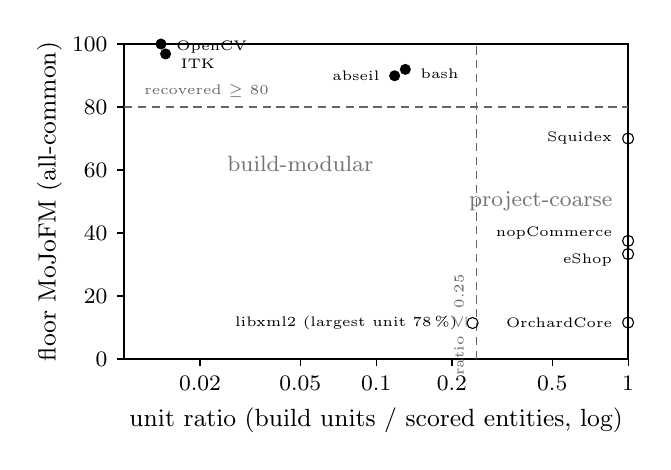
\begin{tikzpicture}
  \draw[thick] (0,0) rectangle (6.4,4);
  \draw (0.963,0) -- (0.963,-0.09); \node[below,font=\footnotesize] at (0.963,-0.09) {0.02};
  \draw (2.237,0) -- (2.237,-0.09); \node[below,font=\footnotesize] at (2.237,-0.09) {0.05};
  \draw (3.2,0) -- (3.2,-0.09); \node[below,font=\footnotesize] at (3.2,-0.09) {0.1};
  \draw (4.163,0) -- (4.163,-0.09); \node[below,font=\footnotesize] at (4.163,-0.09) {0.2};
  \draw (5.437,0) -- (5.437,-0.09); \node[below,font=\footnotesize] at (5.437,-0.09) {0.5};
  \draw (6.4,0) -- (6.4,-0.09); \node[below,font=\footnotesize] at (6.4,-0.09) {1};
  \draw (0,0) -- (-0.09,0); \node[left,font=\footnotesize] at (-0.09,0) {0};
  \draw (0,0.8) -- (-0.09,0.8); \node[left,font=\footnotesize] at (-0.09,0.8) {20};
  \draw (0,1.6) -- (-0.09,1.6); \node[left,font=\footnotesize] at (-0.09,1.6) {40};
  \draw (0,2.4) -- (-0.09,2.4); \node[left,font=\footnotesize] at (-0.09,2.4) {60};
  \draw (0,3.2) -- (-0.09,3.2); \node[left,font=\footnotesize] at (-0.09,3.2) {80};
  \draw (0,4) -- (-0.09,4); \node[left,font=\footnotesize] at (-0.09,4) {100};
  \node[below,font=\small] at (3.2,-0.5) {unit ratio (build units / scored entities, log)};
  \node[rotate=90,font=\small] at (-0.95,2) {floor MoJoFM (all-common)};
  \draw[densely dashed,black!60] (4.473,0) -- (4.473,4);
  \node[anchor=south east,rotate=90,font=\tiny,black!60] at (4.473,1.2) {ratio $\le$ 0.25};
  \draw[densely dashed,black!60] (0,3.2) -- (6.4,3.2);
  \node[anchor=south west,font=\tiny,black!60] at (0.132,3.2) {recovered $\ge$ 80};
  \node[font=\footnotesize,black!55] at (2.237,2.48) {build-modular};
  \node[font=\footnotesize,black!55] at (5.29,2) {project-coarse};
  \fill (3.435,3.597) circle (2pt);
  \node[anchor=east,font=\tiny] at (3.365,3.597) {abseil};
  \fill (3.571,3.678) circle (2pt);
  \node[anchor=west,font=\tiny] at (3.641,3.618) {bash};
  \draw (6.4,1.333) circle (2pt);
  \node[anchor=east,font=\tiny] at (6.32,1.263) {eShop};
  \fill (0.526,3.874) circle (2pt);
  \node[anchor=west,font=\tiny] at (0.596,3.744) {ITK};
  \draw (4.425,0.457) circle (2pt);
  \node[anchor=east,font=\tiny] at (4.355,0.457) {libxml2 (largest unit 78\,\%)};
  \draw (6.4,1.5) circle (2pt);
  \node[anchor=east,font=\tiny] at (6.32,1.6) {nopCommerce};
  \fill (0.468,4) circle (2pt);
  \node[anchor=west,font=\tiny] at (0.538,3.96) {OpenCV};
  \draw (6.4,0.463) circle (2pt);
  \node[anchor=east,font=\tiny] at (6.32,0.463) {OrchardCore};
  \draw (6.4,2.8) circle (2pt);
  \node[anchor=east,font=\tiny] at (6.32,2.8) {Squidex};
\end{tikzpicture}
}
  \caption{The two-regime finding in one view: the autonomous floor's MoJoFM against the build
  graph's unit ratio, which alone needs no reference. Dashed: the post-hoc rule's ratio
  threshold (\rqAdequacyRatioMax{}) and the recovery threshold (\rqTwoRecoveredMin{}). Filled
  markers satisfy the rule; libxml2 fails it through the largest-unit-share clause, not the
  ratio.}
  \label{fig:regimes}
\end{figure}

Table~\ref{tab:rq1} reads as a diagnosis carried by its autonomous columns. On four of the five
C/C++ systems the no-curation floor already sits within a few MoJoFM points of the curated model
(C++ median \rqOneFloorCppMoJo{}). On the four C\#\ systems it does not (median
\rqOneFloorCsMoJo{}): at project granularity the floor \emph{is} the all-singletons partition,
identical to \texttt{dir}, and the curated number is the curator's grouping. The auto-propose
draft is not a reliable autonomous comparator: it recovers abseil exactly
(\rqOneProposeAbseilMoJo{}) but collapses OpenCV into two containers (\rqOneProposeOpencvMoJo{})
and eShop into one (\rqOneProposeEshopMoJo{}). libxml2 marks the boundary from within C++: one
library target gives the build graph nothing to report. a2a tells the other half: the floor's
fine targets sprawl against a 13-cluster reference (ITK floor a2a \rqOneFloorItkAtoA{}), which
curation repairs. ARI (Table~\ref{tab:rq2k}) charges that sprawl in full: the floor scores
\rqOneFloorItkAri{} on ITK and \rqOneFloorAbseilAri{} on abseil although \rqOneFloorItkNested{}\,\%
and \rqOneFloorAbseilNested{}\,\% of its clusters lie inside one reference cluster, a refinement
rather than a misgrouping; the propose draft's merging restores \rqOneProposeItkAri{} and
\rqOneProposeAbseilAri{}. On bash and OpenCV, whose target counts sit near the reference's, the
floor's ARI (\rqOneFloorBashAri{}, \rqOneFloorOpencvAri{}) agrees with MoJoFM. ``Recovers''
therefore means at the granularity of the build targets.

The regime can be read off the build graph without the reference. The floor's \emph{unit ratio}
counts the build units that own at least one scored entity over the scored entities (hence below
Table~\ref{tab:rq1}'s \#Tgt). Across the \rqAdequacyN{} scored systems it correlates with the
floor's MoJoFM at Spearman $\rho=\rqAdequacyRhoRatioMoJo{}$ (bootstrap 95\,\% interval
$[\rqAdequacyRhoCiLo{}, \rqAdequacyRhoCiHi{}]$; $\rqAdequacyRhoRatioAtoA{}$ with a2a) and its
TurboMQ at $\rho=\rqAdequacyRhoMqMoJo{}$. The post-hoc rule ``unit ratio
$\le\rqAdequacyRatioMax{}$ and largest-unit share $\le\rqAdequacyLargestMax{}$'' declares
\rqAdequacyAdequateCount{} systems build-modular (ITK, abseil, OpenCV, bash) and
\rqAdequacyInadequateCount{} not (every C\#\ system at ratio 1.0; libxml2's one library holds
\rqAdequacyLibxmlLargestShare{} of the files), and agrees with a floor MoJoFM of at least
\rqTwoRecoveredMin{} on \rqAdequacyRuleAgreement{} systems (Fig.~\ref{fig:regimes}). The
separation is not knife-edge: the ratio threshold can sit anywhere in
$[\rqAdequacyRatioIntervalLo{}, \rqAdequacyRatioIntervalHi{})$ without changing a call, but
re-selecting both thresholds leave-one-system-out predicts \rqAdequacyLooCorrect{} and misses
\rqAdequacyLooWrong{}, the one system the largest-unit clause exists for (intervals, the
ratio-only variant, Tier-B calls: \trDiagnostic{}). The rule is deliberately simple and a hypothesis for the extension corpus
(\S\ref{sec:threats}). It calls none of the \rqAdequacyTierBSystems{} unreferenced Tier-B
systems build-modular; fmt (\rqAdequacyFmtUnits{} CMake targets over \rqAdequacyFmtEntities{}
files) is the project-coarse C++ case the scored corpus lacks.

\subsection{RQ2: Comparison with classical SAR and an LLM baseline}
\label{sec:rq2}

Table~\ref{tab:rq2} gives every technique the same graph and reference on both metrics. Against
the five all-common classical baselines the floor leads strictly on \rqTwoFloorMoJoWins{} systems
by MoJoFM (\rqTwoFloorMoJoWinsOrTies{} with ties; on C\#\ floor and \texttt{dir} coincide) and on
\rqTwoFloorAtoAWins{} by a2a; the propose draft on \rqTwoProposeMoJoWins{} and
\rqTwoProposeAtoAWins{}. On C\#\ the classical techniques collapse into one or two blobs through
the shared building-block projects, and on libxml2 everything sits at the floor. The curated
model leads strictly on \rqTwoPipelineMoJoWins{} systems by MoJoFM and \rqTwoPipelineAtoAWins{} by
a2a against the classical set, and on \rqTwoPipelineMoJoWinsAll{} and \rqTwoPipelineAtoAWinsAll{}
against every displayed baseline including ARC and the LLM. On C\#\ that margin is curation,
sighted on three systems (Table~\ref{tab:corpus}).

Under the post-hoc ARI of Table~\ref{tab:rq2k} the picture sharpens rather than changes. No
classical technique exceeds \rqTwoSarAriMax{} (\rqTwoSarAriMaxWhere{}) on any system, and the
C\#\ classical cells sit at chance. The curated model leads on \rqTwoPipelineAriWins{} systems,
the propose draft on \rqTwoProposeAriWins{}, and the floor on \rqTwoFloorAriWins{}, its
over-splitting of the two finest build graphs now visible. On the autonomous rows no difference
reaches significance, which at $n=\rqTwoFriedmanFloorN{}$ speaks to power, not to equivalence.
The Friedman omnibus does not reject equality with the floor
(MoJoFM $p=\rqTwoFriedmanFloorP$, a2a $p=\rqTwoFriedmanFloorAtoAP$, $n=\rqTwoFriedmanFloorN$) or
with the propose draft ($p=\rqTwoFriedmanProposeP$ and \rqTwoFriedmanProposeAtoAP{}) in place of
the curated row, and no Holm-corrected pairwise Wilcoxon or Nemenyi comparison separates either
row from any technique (\trStats{}). The curated row's omnibus ($p=\rqTwoFriedmanP$; differs from
\rqTwoPosthocDiffers{} after correction) is descriptive only.

By the post-hoc bands no classical technique reaches the recovery threshold on any of the four
C\#\ systems: \rqTwoCsClassicalFailed{} of \rqTwoCsClassicalCells{} technique--system cells fail,
and the \rqTwoCsClassicalPartial{} partial ones (\rqTwoCsClassicalPartialList{}) stay far below
\rqTwoRecoveredMin{}. The LLM is the strongest autonomous comparator: it recovers
\rqTwoLlmCsRecovered{} (\rqOneLlmEshopMoJo{}), is partial on \rqTwoLlmCsPartial{}, fails on
\rqTwoLlmCsFailed{}, varies across reruns on Squidex (Table~\ref{tab:rq2}), and was not run on
ITK, whose file graph exceeds the input budget fourfold (no call was made). ARC did not
reproduce either~\cite{link2019value}. SARIF~\cite{zhang2023sarif} and FCA~\cite{teymourian2022fca}
published scores against the very references used here for bash, ITK, and libxml2
(\trPublished{}). Our floor sits above both on bash and ITK, and SARIF's own ACDC run sits below
our ACDC row, so our inputs do not handicap the baselines. On libxml2 SARIF's text-and-folder
fusion beats every structural partition we score.

\subsection{RQ3: Ablation}
\label{sec:rq3}

Ablations are paired per system (Table~\ref{tab:rq1}). \emph{Curation (A2):} on the all-common
set curation adds \rqThreeCurationLiftCpp{} MoJoFM points on C++ and \rqThreeCurationLiftCs{} on
C\#\ (paired $r=\rqThreeCurationRankBiserialCs{}$, $p=\rqThreeCurationWilcoxonP{}$; the two
language groups' floors differ with Cliff's $\delta=\rqThreeFloorCliffsCppVsCs{}$).
\emph{Evidence layers (A1):} L0 alone yields
most container edges and the symbol layer the remainder (per layer: \trAblation{}).
\emph{Declared dependencies never dropped (A5):} at the default threshold of 3 the rule saves
\rqThreeAfiveOperatingEdgesSaved{} edges on \rqThreeAfiveOperatingSystemsChecked{} systems,
because every declared dependency clears the bar on its base weight. At 8, where a curator might
silence noisy include edges, a scalar filter cuts declared edges it cannot tell from noise,
removing \rqThreeAfiveEshopEdgesSaved{} of eShop's container edges (edge counts move on
\rqThreeAfiveWilcoxonN{} systems, paired $r=\rqThreeAfiveRankBiserial{}$,
$p=\rqThreeAfiveWilcoxonP{}$; reference recall falls by \rqThreeAfiveRefRecallDropList{} on the
\rqThreeAfiveRefRecallSystems{} systems where it is scored, too few to test). Thresholding (A3)
barely moves the edge set at the operating point and visibility down-weighting (A4) is inert.
\emph{Names, never structure (A6, A7):} read as the LLM-does-structure arm, the RQ2 LLM runs
recover a competitive partition on small systems and beat the curated model on
\rqThreeSixLlmGtPipelineList{}. But the deterministic pipeline matches or beats them on
\rqThreeSixPipelineGeLlm{} of the systems they completed (median LLM MoJoFM
\rqThreeSixLlmMedianMoJo{}), and ITK did not fit one prompt. An adversarial provider that renames every
element perturbs \rqThreeSevenMaxStructuralDelta{} relationships on
\rqThreeSevenSystemsChecked{} systems, confirming the invariant of \S\ref{sec:enrich}.

\subsection{RQ4: Reproducibility and stability}
\label{sec:rq5}

Byte-identical regeneration is a tested invariant (\S\ref{sec:generate}), the contrast with ARC and
the LLM baseline. What we measure is survivor-partition agreement under code change (A8). After
20\,\% entity turnover the per-entity rules keep every surviving entity in its cluster
(\rqFivePipelineChurn{} on all eight systems), as does \texttt{dir} (\rqFiveDirChurnMedian{}),
whereas ACDC, a global optimiser, reshuffles survivors on every system (median
\rqFiveAcdcChurnMedian{}, down to \rqFiveAcdcChurnWorst{} on abseil). Rules bind identities rather
than graph optima, so the contrast is one of semantics, not of correctness: a frozen ACDC
partition would keep its survivors too, but assigns nothing to new entities and carries no
evidence. A8 does not say the model is still \emph{right} later: new targets surface as
\texttt{needs-curation} singletons for the human, which \S\ref{sec:rq6} counts on real history.

\subsection{RQ5: Drift detection and governance}
\label{sec:rq6}

\paragraph{Seeded mutations and degradation (correctness).} We injected \rqSixMutationCount{}
labelled changes (\rqSixOperatorCount{} operators: add and remove a dependency; add, remove,
rename, and merge a target) into the \emph{build files} of checkout copies of
\rqSixMutationSystems{} systems across three build idioms. We ran the whole pipeline on each and
scored the report against the label, one finding per vanished or new target, edge, rename, or
violation. The report covered \rqSixMutationsDetected{} mutations fully, with precision
\rqSixPrecision{}, recall \rqSixRecall{}, \rqSixFpPerPr{} false findings per simulated pull
request, renames classified as renames (accuracy \rqSixRenameAccuracy{}), and a one-line alias
pin silencing the drift in \rqSixAliasSurvival{} pinned reruns (per operator: \trDrift{}).
Inducing evidence degradation on the \rqSixDegradationSystems{} systems scored before Squidex
joined (semantic toolchain lost; 10\,\% and 30\,\% of targets starved of L0 evidence; build-graph
extractor lost) produces \rqSixWouldBeFalse{} would-be-false ``disappeared'' findings, of which
the stopping rules reclassify all of them as labelled coverage gaps (suppression rate
\rqSixSuppressionRate{}), where a
coverage-naive differ reports every one as change (exact McNemar $p\rqSixMcNemarP$).

\paragraph{Change and evidence loss at once.} Neither arm tests that degradation never hides
erosion, so we replayed the \rqSixCombMutations{} mutations on \rqSixCombSystems{} systems
with each degradation mode induced on the mutated run, plus an adversarial mode that starves
exactly the targets the mutation touches, and classified, per mode, each of the
\rqSixCombFindings{} expected findings as named drift, coverage gap, advisory-only, or silent (\trDrift{}). Under
targeted starvation \rqSixCombStarveMutatedDrift{} are drift, \rqSixCombStarveMutatedGap{} gaps,
and \rqSixCombStarveMutatedAdvisory{} advisory only. The experiment also found a hole: with the
build-graph extractor lost entirely, an added or renamed target was reported nowhere and the run
was not even advisory (\rqSixCombPrefixSilentTotal{} silent findings in that mode), because an empty
first-party target set counted as fully covered. After changing that convention (nothing covered,
advisory), \rqSixCombSilentTotal{} silent findings remain, the \rqSixCombLoseLZeroAdvisory{}
former ones are advisory, and no mode produced a false finding. The claim survives in a weaker
form: erosion is never hidden, but under heavy evidence loss it is often visible only as a warning
that evidence dropped.

\paragraph{Real history.} We then ran the detector over \rqSixHistPairs{} consecutive release pairs
of \rqSixHistSystems{} systems (libxml2, nopCommerce, Squidex), fixed in advance rather than
selected by changelog, with the committed rules held constant across each pair (per pair:
\trDrift{}). The \rqSixHistCommits{} commits, \rqSixHistBuildCommits{} of them touching build
files, yielded \rqSixHistFindings{} findings and \rqSixHistCoverageGaps{} coverage gaps;
\rqSixHistPairsZero{} pairs with build-file churn produced none. Of the \rqSixHistNewTargets{} first-party targets the releases added, the rules left
\rqSixHistNewUnmapped{} unmapped, as expected: the Squidex and nopCommerce overlays post-date both
releases, and libxml2's predate them. Two raters labelled each finding independently: both
called \rqSixHistArchitectural{} architectural, \rqSixHistNonArchitectural{} non-architectural and
\rqSixHistNoise{} extraction noise, with raw agreement \rqSixHistLabelsAgree{} and pooled
Cohen's $\kappa$ of \rqSixHistLabelsKappa{}.

\subsection{RQ6: Performance and scalability}
\label{sec:rq7}

Across \rqSevenSystems{} systems spanning \rqSevenMinKloc{}--\rqSevenMaxKloc{}\,KLOC, the cold
end-to-end run (CMake configure, Doxygen, and Roslyn included) stays within the 30-minute budget
on \rqSevenColdBudget{} systems and the warm rerun within the 3-minute budget on
\rqSevenWarmBudget{} (median speedup \rqSevenMedianSpeedup$\times$; log--log slope
\rqSevenScalingSlope{} against KLOC; peak RSS \rqSevenMaxPeakRssGb{}\,GB; per system:
\trPerf{}). The exception is ITK: its cold run takes \rqSevenItkColdMin{} minutes,
\rqSevenItkDoxygenSharePct{}\,\% of it in Doxygen's XML pass, against \rqSevenItkWarmMin{} warm.
At this size the L2 layer misses the per-commit budget; an L0-only run would take about
\rqSevenItkLZeroImpliedMin{} minutes (an estimate, not a measurement).

\subsection{RQ7: Curation value under blinding}
\label{sec:rq9}
%% GENERATED by analysis/make_tables.py from results.csv -- DO NOT EDIT BY HAND.
\begin{table}[t]
  \centering
  \caption{RQ7 blind curation (terms: \S\ref{sec:design}; all-common projection; best SAR = best of ACDC/WCA/LIMBO, \texttt{dir} coinciding with the floor here). R$_1$ vs.\ R$_2$ = the reference authors' agreement, an inter-rater baseline; Edge-F1 = container-edge F1; $\kappa$ = raw Cohen's $\kappa$ on rater labels; confl. = rater clusters cutting a reference boundary; the consensus row is a sensitivity re-score, the second-curator row the curator-variance arm.}
  \label{tab:rq9}
  \footnotesize\setlength{\tabcolsep}{2.2pt}
  \begin{tabular}{@{}lll rrl@{}}
    \toprule
    System & Row & Kind & MoJo & a2a & Edge-F1\,/\,$\kappa$ \\
    \midrule
    eShop & no-curation floor & det. & 33.3 & 80.8 & -- \\
     & best SAR (LIMBO) & det. & 26.7 & 85.9 & -- \\
     & \textbf{blind curator} & expr. & \textbf{86.7} & \textbf{95.8} & 0.63 \\
     & \quad second blind curator (R-B) & expr. & 66.7 & 90.8 & 0.56 \\
     & \quad curator vs.\ curator agreement & agr. & 80.6 & 93.9 & ARI\,0.75 \\
     & \quad vs.\ consensus & expr. & 75.0 & 92.0 & 0.55 \\
     & R$_1$ vs.\ R$_2$ agreement & agr. & 66.5 & 89.7 & $\kappa$\,0.00; 0\,confl. \\
    \midrule
    Squidex & no-curation floor & det. & 70.0 & 92.0 & -- \\
     & best SAR (LIMBO) & det. & 60.0 & 93.0 & -- \\
     & \textbf{blind curator} & expr. & \textbf{70.0} & \textbf{95.8} & 0.67 \\
     & R$_1$ vs.\ R$_2$ agreement & agr. & 54.5 & 86.3 & $\kappa$\,0.39; 0\,confl. \\
    \bottomrule
  \end{tabular}
\end{table}


On both systems the reference-blind curator lands above every classical technique on a2a and
above ACDC, WCA, and LIMBO on MoJoFM (Table~\ref{tab:rq9}): \rqNineEshopCuratorMoJo{} MoJoFM on eShop and \rqNineSquidexCuratorMoJo{} on
Squidex (a2a \rqNineEshopCuratorAtoA{} and \rqNineSquidexCuratorAtoA{}; container-edge F1
\rqNineEshopCuratorEdgeFone{} and \rqNineSquidexCuratorEdgeFone{}), \rqNineEshopOverBestSarMoJo{}
and \rqNineSquidexOverBestSarMoJo{} points above the best of ACDC, WCA, and LIMBO. The
informative comparison is against the reference, which on eShop
both raters, who never saw it, re-derive at \rqNineEshopRaterRefMoJoMin{} MoJoFM or better
(aligned $\kappa\ge$\rqNineEshopRaterRefKappaAlignedMin{}): it is not one author's opinion, and
the curator is at least as close to it as its re-derivers.

The plan's raw-$\kappa$ flag fired on both systems (\rqNineEshopKappa{}, \rqNineSquidexKappa{}),
but raw $\kappa$ scores exact label match. Label-free, eShop's raters agree (aligned $\kappa$
\rqNineEshopKappaAligned{}) and Squidex's disagree (\rqNineSquidexKappaAligned{}). On both systems
not one rater cluster cuts across a reference boundary: the partitions nest, and every
disagreement is about altitude, where the projects' documentation is silent (\trCuration{}).
eShop's sighted curation scored \rqNineEshopNonBlindMoJo{}; the blind curator scores
\rqNineEshopLeakageDelta{} points \emph{higher}, so reference access is not what carried the
sighted score, though curator differences remain a confound. The raters' consensus sits at a
coarser altitude (\rqNineEshopCuratorVsConsensusMoJo{} against it) and is a sensitivity row, not
a second reference. On Squidex the raters settled on fine granularity
(\rqNineSquidexConsensusClusters{} clusters over 15 projects), so the singleton floor is strong
(\rqNineSquidexFloorMoJo{}) and ACDC, WCA, and LIMBO fall below it. On the all-common projection
(13 of 15 reference projects; two have no first-party dependency and are unseen by the edge-only
techniques) the curator ties the floor on MoJoFM and lifts a2a from \rqNineSquidexFloorAtoA{} to
\rqNineSquidexCuratorAtoA{}; on the full reference it scores
\rqNineSquidexCuratorFullRefMoJo{}/\rqNineSquidexCuratorFullRefAtoA{}.

Effort was \rqNineEshopMinutes{} minutes and \rqNineEshopOps{} editor operations for eShop,
\rqNineSquidexMinutes{} and \rqNineSquidexOps{} for Squidex, whose curator worked in two
sittings around a GUI defect in that packet and inspected projects several times eShop's
size. A second, equally blind eShop curator (\rqNineEshopSecondCuratorCode{}), the one
measurement of curator variance, took \rqNineEshopSecondCuratorMinutes{} minutes over two
sittings and scored \rqNineEshopSecondCuratorMoJo{} MoJoFM (a2a
\rqNineEshopSecondCuratorAtoA{}): above every classical technique but
\rqNineEshopCuratorMoJoSpread{} points below the first curator, the two agreeing at aligned
$\kappa$ \rqNineEshopCuratorPairKappaAligned{} (\trCuration{}). No curator kept a group from the
\cli~\texttt{propose} draft (\rqNineEshopProposeDerivedPct\% and
\rqNineSquidexProposeDerivedPct\%), the same null the propose row of Table~\ref{tab:rq1} shows.
